\documentclass[a4paper,10pt, oneside]{article}
\usepackage[utf8]{inputenc}
\usepackage[spanish]{babel}
\usepackage[style=ieee,backend=bibtex]{biblatex}
\usepackage{graphicx}
\usepackage{amsmath}
\usepackage{pgfplots}
\usepackage{lineno}
\usepackage{amsmath}
\usepackage[top=1in, bottom=1.25in, left=1.25in, right=1.25in]{geometry}
\usepackage{caption}
\usepackage{bytefield}
\usepackage{amsmath}
\usepackage{csquotes}
\usepackage{svg}
\usepackage{lscape}
\usepackage{draftwatermark}
\usepackage[linesnumbered,ruled]{algorithm2e}


\bibliography{informe_final}
	
\begin{document}
	
\begin{titlepage}
	\centering
	
\includegraphics[width=0.25\textwidth]{../Universidad_del_Litoral}\par\vspace{1cm}
	{\scshape\LARGE Universidad Nacional del Litoral \par}
	\vspace{1cm}
	{\scshape\Large Proyecto Final de Carrera\par}
	\vspace{1.5cm}
	{\huge\bfseries Diseño de un sistema de detección de anomalías en redes de computadoras.\par}
	\vspace{4cm}
	{\huge\bfseries Informe Final\par}
	\vfill
	
	{\Large \itshape Pineda Leandro\par}
	
	
	% Bottom of the page
	\large Córdoba\par
	{\large \today\par}	
\end{titlepage}

\modulolinenumbers[5]
\linenumbers

\clearpage\mbox{}\clearpage

\section{Introducción}
En la actualidad, \textit{BigData} es uno de los tantos conceptos de moda en el mundo informático. Este se usa para hacer referencia a grandes colecciones de datos que pueden crecer a volúmenes enormes y a un ritmo tan alto que resulta difícil o imposible manejarlos con las herramientas tradicionales, como las bases de datos relaciones convencionales. El desafío que presenta el \textit{BigData} no solo está limitado a los aspectos técnicos de almacenar cantidades masivas de datos, sino en cómo obtener de estos información relevante que permitan asistir a la toma de decisiones.
Este concepto comenzó a tomar fuerza a principios del año 2000 cuando Doug Laney, vicepresidente y analista distinguido de Gartner\footnote{Gartner Inc. es una empresa consultora y de investigación de las tecnologías de la información con sede en Stamford, Connecticut, Estados Unidos}, caracterizó al \textit{BigData} mediante tres V:
\begin{itemize}
	\item Volumen: Las organizaciones recolectan cantidad masivas de datos de diversas fuentes (transacciones, social-media, sensores, etc). En el pasado, almacenar tal volumen de datos hubiese sido un problema, pero nuevas tecnologías como \textit{Hadoop} surgieron para hacer frente al desafío.
	\item Velocidad: Los datos se generan cada vez a mayor velocidad, y deben ser manejados en un tiempo aceptable. Etiquetas RFID, sensores y dispositivos IoT, entre otros, hacen que sea necesario procesar estos flujos de datos rápidamente.
	\item Variedad: Los datos vienen en todo tipo de formatos (estructurados, semi-estructurados o sin estructura).
\end{itemize}

Dependiendo de la necesidad de negocios particular de cada empresa o entidad y la naturaleza de los datos, una de las tres V descritas puede ser más importante que las otras. Si se quiere hacer un pronóstico para cierta actividad, por ejemplo, será necesario contar con grandes volúmenes de datos del pasado. Por el contrario, si es necesario entender cómo varía cierto patrón en los datos en una ventana de tiempo cercana a la presente, será necesario procesarlos de manera instantánea, obviando tal vez su almacenamiento dado que contar con esta información del pasado no genera valor alguno, o su almacenamiento es inviable.
\

De la misma manera que surgieron técnicas para procesar datos almacenados en soportes distribuidos como \textit{MapReduce}\cite{Dean:2004:MSD:1251254.1251264}, donde grandes volúmenes de información permanecen estáticos y pueden ser accedidos de manera aleatoria, la necesidad del procesamiento \textit{on-line} de flujos de datos originó el surgimiento de un conjunto de técnicas conocido como \textit{Data Streaming}. Haciendo uso de las mismas, es posible identificar en tiempo real la ocurrencia de ciertos patrones de interés en los flujos de datos, sin necesidad de almacenar su totalidad para procesarlos. Estas técnicas, que serán desarrolladas más adelante, tienen características especiales que hacen que su implementación sea sencilla, de forma que no demanden grandes cantidad de recursos computacionales y no introduzcan así demoras en la producción de resultados (pero, en algunos casos, al coste de sacrificar precisión).

Las técnicas de \textit{Data Streaming} pueden aplicarse en diversos campos. En particular, la detección en tiempo real de ciertos patrones en los flujos de datos de una red de computadoras (que en algunos casos pueden ayudar a determinar incidentes tales como escaneo de puertos, ataques de denegación de servicio, expansión de \textit{malware} entre otros), es de vital importancia para salvaguardar la integridad de dicha infraestructura informática. Estas anomalías pueden encontrarse analizando los flujos de datos y llevando cuenta de todos los paquetes que atraviesan los puntos de acceso a la red. En la capa de transporte, el protocolo TCP (que provee conexión host a host sobre IP) provee información suficiente para identificar estos patrones. Para llevar a cabo el análisis en tiempo real de los segmentos TCP que son transportados, utilizaremos el modelo de \textit{Data Streaming}.

Además, se describirá la arquitectura de un sistema basado en microservicios que implementa un algoritmo basado en \textit{sketches} y las tecnologías empleadas para su desarrollo. Finalmente, se mostrarán los resultados de las pruebas realizadas.

\clearpage\mbox{}\clearpage

\section{Data Streaming}

Antes de comenzar a desarrollar el modelo de \textit{Data Streaming}, es necesario introducir dos definiciones que con frecuencia son usadas indistintamente debido a su similitud, pero que significan conceptos diferentes: \textbf{\textit{Streaming Data}} hace referencia a los datos que son generados continuamente por un conjunto de orígenes de datos de forma simultáneamente. Estos datos son de diferente naturaleza como logs de cliente usando aplicaciones móviles o web, compras en plataformas virtuales, actividad de usuarios en juegos, información de redes sociales, telemetría de dispositivos, entre otros. Por otra parte, \textbf{\textit{Data Streaming}} o \textbf{\textit{Stream Processing}} hace referencia a las técnicas de procesamiento utilizada para \textit{Streaming Data}. En el paradigma de \textit{Streaming Data}, los datos son procesados directamente mientras son producidos o recibidos. Antes del surgimiento del \textit{Stream Processing}, la información era almacenada en bases de datos, sistemas de archivos u otra forma de almacenamiento masivo para luego ser procesada. El termino \textit{BigData} hace referencia a este otro paradigma, en el cual grandes volúmenes de datos permanecen estáticos en algún soporte de almacenamiento masivo, mientras que diferentes algoritmos permiten realizan consultas o ejecutar procesos en la medida que lo necesitan.

\begin{figure}[htbp]
	\centering
	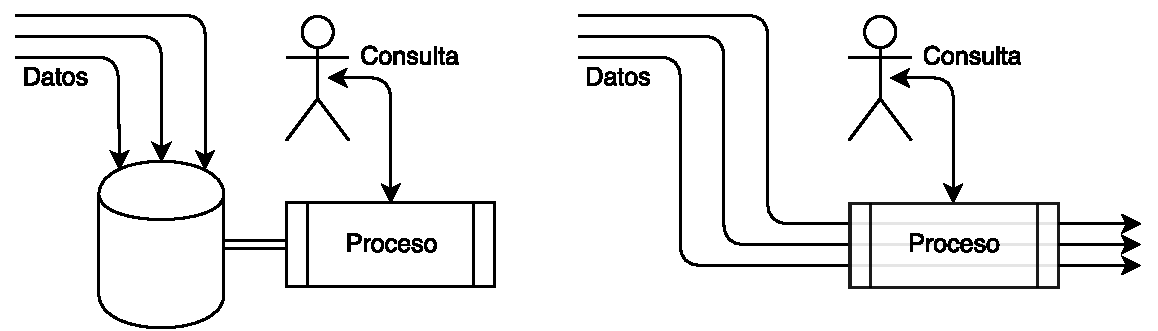
\includegraphics[width=0.8\textwidth]{./graph/bigdata_vs_streamingdata.pdf}
	\caption{Gráfica conceptual de BigData vs Streaming Data}
	\label{fig:bigdata_vs_streamingdata}
\end{figure}

En la figura \ref{fig:bigdata_vs_streamingdata} (izquierda) puede observarse un diagrama esquematizado del enfoque clásico de \textit{BigData}, donde todos los datos son almacenados en algún tipo de base de datos, y luego se realizan consultas sobre estos mediante algún proceso particular que permita extraer información relevante. A la derecha de la figura \ref{fig:bigdata_vs_streamingdata} se puede observar un esquema de las partes relevantes del enfoque de \textit{Data Streaming}; la diferencia más importante entre estos dos paradigmas es no existe la persistencia de datos. Las consultas se realizan sobre datos `en movimiento', en lugar de utilizar datos estáticos.

\

En los últimos años, los avances en las tecnologías de hardware han posibilitado colectar datos de forma continua. Transacciones que hacemos en nuestra vida cotidiana como el uso de una tarjeta de crédito, un teléfono o navegar la web generan grandes cantidades de datos. De la misma manera, los avances en las tecnologías de la información hicieron que los flujos de información en las redes IP sean cada vez mayores. En muchos casos, los datos generados pueden ser minados para obtener información relevante que puede ser utilizada en gran cantidad de aplicaciones. Sin embargo, cuando el volumen de datos es muy grande, se presentan algunos problemas:

\begin{itemize}
	\item No es posible un procesamiento eficiente de los datos usando métodos que requieran varias pasadas sobre el \textit{dataset} (por ejemplo, aquellos usados en \textit{BigData}). En su lugar, dada la velocidad a la que se producen estos datos, uno puede permitirse procesar cada dato a lo sumo una vez, lo que impone ciertas restricciones en la implementación de los algoritmos de procesamiento. Por lo tanto, las técnicas de procesamiento de \textit{Streaming Data} deben ser diseñadas de forma que los algoritmos cumplan su cometido con una única pasada por el conjunto de datos.
	\item En muchos casos, el proceso de minar \textit{Streaming Data} tiene una componente temporal inherente: los datos puede evolucionar a medida que pasa el tiempo. Este comportamiento de los \textit{streams} de datos es llamado \textit{localidad temporal}\cite{Aggarwal:2006:DSM:1196418}. Por esta razón, una adaptación directa de los algoritmos de una pasada para minar \textit{Streaming Data} puede no se una solución efectiva para esta tarea. Estos deben diseñados cuidadosamente haciendo foco en la evolución de los datos que están siendo procesados.
\end{itemize}

Antes de presentar algunas de las técnica existentes para procesar \textit{streams} de datos, es conveniente introducir la notación que utilizada para describirlos.

\subsection{El modelo de Data Streaming}
En el modelo de \textit{Data Streaming}, los datos que van a ser procesados no están disponibles para ser accedidas aleatoriamente desde disco o memoria, sino que llegan como uno o mas flujos continuos de datos. Los \textit{streams} de datos son diferentes de los modelos relacionales convencionales en varios aspectos: 
\begin{itemize}
	\item Los elementos del \textit{stream} deben ser procesados de manera \textit{online}, esto es, sin ser persistidos en ningún soporte de almacenamiento.
	\item Los sistemas que procesan los datos no tienen control sobre el orden en los elementos de la entrada.
	\item Los \textit{stream} de datos pueden ser infinitos.
	\item Una vez que un elemento es procesado, este se descarta.\footnote{En algunas aplicaciones los elementos pueden ser almanacenados para procesamiento posterior, pero en un modelo de \textit{streaming} "puro" los elementos son procesados una única vez.}
\end{itemize}

Otra característica de este modelo que es conveniente remarcar se relaciona con las consultas a los datos procesados: podemos hacer una distinción entre \textit{consultas únicas} y \textit{consultas continuas}\cite{Terry:1992:CQO:141484.130333}. Las primeras (como aquellas que se hacen mediante un DBMS tradicional) son evaluadas una vez sobre un conjunto de datos en un instante de tiempo particular (los datos no cambian durante la duración de la consulta). La consultas continuas, por otro lado, son evaluadas continuamente mientras el \textit{stream} de datos esta ocurriendo. Las respuestas a estas consultas pueden ser almacenadas y actualizadas en la medida que llegan nuevos flujos de datos, o pueden ser origen de otro \textit{stream} de datos.

\

Existen tres modelos diferentes para describir \textit{Streaming Data}. Supongamos que se quiere analizar un \textit{stream} de datos que está siendo generado por cierta aplicación. Los datos $t_1, t_2, \dots$ llegan secuencialmente, elemento por elemento, y describe una señal $\mathbf{a}$ como una función unidimensional $\mathbf{a}: [1 \dots N] \rightarrow R$. Los modelos difieren en cómo los $t_i$ describen a la señal $\mathbf{a}$.

\subsubsection{Modelo de series de tiempo}
Dado los elementos $t_i$ que se presentan en orden creciente de $i$, la señal $\mathbf{a}$ esta conformada por $\mathbf{a}[i]=t_i$. Este modelo es adecuado para ser usado cuando los elementos del \textit{stream} forman series de tiempo. Por ejemplo, si se quiere realizar observaciones sobre el volumen de transacciones del NASDAQ cada minuto.
\subsubsection{Modelo de caja registradora}
En este modelo, los $t_i$ modifican el estado de los $\textbf{a}[j]$. Podemos pensar cada elemento $t_i$ como una tupla $t_i = (j, I_i)$, $I_i \geq 0$ que provoca una actualización $\textbf{a}_i[j] = \textbf{a}_{i-1} [j] + I_i$ donde $\textbf{a}_i$ es el estado de la señal luego de procesar el i-ésimo elemento del \textit{stream}. Es importante observar que múltiples $t_i$ pueden incrementar un $\textbf{a}[j]$ a lo largo del tiempo. Este es tal vez el más popular de los modelos de \textit{streams} de datos. Es útil para aplicaciones como monitoreo de direcciones IP que acceden un servidor, direcciones IP de origen que envían paquete en un enlace dado, etc, dado que la misma dirección IP puede acceder al servidor muchas veces o puede enviar multiples paquetes en un período de tiempo dado.
\subsubsection{El modelo Turnstile}
De la misma forma que en el modelo anterior, los $t_i$ actualizan a los $\textbf{a}[j]$. Cada elemento $t_i = (j, U_i)$ produce  $\textbf{a}_i[j] = \textbf{a}_{i-1} [j] + U_i$ donde $\textbf{a}_i$ es la señal luego de la ocurrencia del i-ésimo elemento en el \textit{stream}, y $U_i$ puede ser positivo o negativo. Este modelo es el mas general de todos (notar que es igual al modelo de caja registradora, pero admite valores de $I_i$ negativos). Es apropiado para estudiar situaciones completamente dinámicas donde puede haber inserción y borrado de elementos. 

\

Realizar consultas sobre \textit{streams} de datos presenta desafíos únicos. Dado que los flujos de datos son potencialmente infinitos, la cantidad de espacio de almacenamiento requerido para calcular la respuesta exacta de una consulta acerca de los datos también podría crecer infinitamente. Si bien se han estudiado algoritmos para procesar conjuntos de datos que exceden la memoria principal de una computadora\cite{Vitter:2001:EMA:384192.384193}, estos no son útiles para aplicaciones de \textit{Data Streaming} dado que no soportan consultas continuas y son típicamente muy lentos para generar resultados en tiempo real. El modelo en discusión es aplicable a problemas donde es importante que los resultados de las consultas realizadas se obtengan rápidamente y donde hay grandes volúmenes de datos que están siendo producidos continuamente a gran velocidad. Nuevos datos continúan llegando mientras los datos previos están siendo procesados; el tiempo de cómputo por dato debe ser bajo, de lo contrario, se introduce latencia y el algoritmo no será capaz de procesar los datos en tiempo real. Por este motivo, estos algoritmos deben ser capaces de funcionar haciendo uso únicamente de la memoria principal, sin realizar accesos a disco.

Cuando la cantidad de memoria disponible es finita, no siempre es posible producir respuestas exactas a las consultas realizadas a \textit{streams} de datos (recordemos, potencialmente de duración infinita). Sin embargo, es posible obtener muy buenas aproximaciones a las mismas, que son aceptables cuando no se dispone de la respuesta exacta. Si bien distintos algoritmos para aproximar respuestas a consultas realizadas sobre \textit{streams} de datos han sido estudiados en los últimos años, para este trabajo haremos foco en una estructura de datos conocida como  \textit{sketch}\cite{Alon:1996:SCA:237814.237823}\cite{Flajolet:1985:PCA:5212.5215} debido a las bondades que presentan. Además, introduciremos algunas técnicas de conteo de gran utilidad para resolver ciertos problemas de minado de \textit{Streaming Data}.



\section{El problema de los elementos frecuentes}
El problema de los elementos frecuentes es uno de los más estudiados desde los años 80 dada su importancia en el minado de \textit{Data Streams}. Muchas de las técnica utilizadas en este área se basan directa o indirectamente en encontrar elementos frecuentes en \textit{streams} de datos. Enunciado de forma sencilla, el problema consta en determinar aquellos elementos que tienen mayor frecuencia de ocurrencia dado un \textit{stream} de elementos. Aquí asumimos que el \textit{stream} es lo suficientemente largo como para que las soluciones convencionales, intensivas en uso de recursos, como ordenar los elementos o mantener un contador por cada uno estos, sean inviables. 
\

Podemos dividir los algoritmos para encontrar elementos frecuentes en tres clases. Los \textbf{algoritmos basados en conteo} operan sobre un subconjunto de elementos y mantienen un contador asociado a los mismos. Por cada entrada nueva, el algoritmo decide si actualizar o no el contador del elemento, y de hacerlo, con que valor lo afecta. 
La segunda clase de algoritmos, que no será analizada en este documento, es una derivación de los \textbf{algoritmos de cuantiles}; el problema de encontrar cuantiles en la distribución de un \textit{stream} de datos nos permite encontrar elementos frecuentes.
Finalmente, los algoritmos basados en \textbf{\textit{sketchs}} utilizan proyecciones lineales aleatorias de las entradas\cite{Cormode:2008:FFI:1454159.1454225} (vistas como vectores de características) y por lo tanto, no almacenan explícitamente los elementos de entrada. Estos últimos tienen ciertas propiedades que son de gran utilidad para procesamiento de múltiples \textit{streams} de datos.

\subsection{Elementos frecuentes en data streams}\label{elementos_frecuentes_en_datastreams}
Antes de describir los algoritmos para encontrar elementos frecuentes es necesario enunciar formalmente el problema.

\subsubsection{Elementos frecuentes}\label{elementos_frecuentes} Dado un stream $S$ de $n$ elementos $t_1$, $t_2$, \dots, $t_n$, la frecuencia del elemento $i$ es $f_i = |\{j|t_j=i\}|$ (es decir, la cantidad de índices $j$ donde el $j$th elemento es $i$). Los $\phi$ elementos frecuentes están dados por $\{i|f_i>\phi n\}$.

\textbf{Ejemplo}: El stream $S=\{a,a,b,a,c,b,a\}$ tiene $f_a=4$, $f_b=2$ y $f_c=1$. Para $\phi=0.2$ los elementos frecuentes son $a$ y $b$.

\

Encontrar exactamente los $\phi$ elementos frecuentes puede ser costoso en términos de recursos: un algoritmo que resuelve el problema de los elementos frecuentes debe usar una cantidad lineal de espacio\cite{Cormode:2010:MFF:1731351.1731356}. Para relajar el requerimiento de recursos se utiliza una aproximación a la solución del problema.

\subsubsection{$\epsilon$-aproximación de elementos frecuentes} 
Dado un stream $S$ de $n$ elementos una $\epsilon$-aproximación de los elementos frecuentes esta dada por el conjunto $F$ tal que todos los elementos $i \in F$ tengan frecuencia $f_i > (\phi - \epsilon)n$, y que no exista $i \notin F$ con $f_i > \phi n$. Dicho de otra manera, una $\epsilon$-aproximación de los elementos frecuentes consiste en encontrar todos los elementos con frecuencia mayor o igual a $\phi n$, de los cuales ninguno tiene frecuencia menor que $(\phi - \epsilon) n$.

\subsubsection{Estimación de la frecuencia de un elemento}
Un problema relacionado a los anteriores consiste en estimar la frecuencia de los elementos al momento que se están procesando los datos. Dado un stream $S$ de $n$ elementos con frecuencias $f_i$, el problema de estimación de frecuencia consiste en procesar el stream de forma que para cualquier $i$ se pude obtener un $\hat{f_i}$ tal que $\hat{f_i} \leq f_i \leq \hat{f_i}+\epsilon n$.

\

Los elementos frecuentes, también llamados \textbf{heavy hitters}, son problemas muy estudiados por sus aplicaciones en bases de datos y \textit{data streaming}. Son también conocidos como \textit{top-k}, \textit{frequent items}, \textit{elephants} o \textit{iceberg queries}. Usualmente, cuando se busca identificar estos elementos de forma \textit{on-line} se trabaja en ventanas de tiempo acotadas o épocas de detección con el objetivo de encontrar \textit{heavy hitters} en momentos particulares del tiempo. Otro patrón que resulta de interés para caracterizar los datos en tránsito son los \textbf{heavy changers}: podemos decir que los \textit{heavy changers} son aquellos elementos que varían de forma significativa en épocas consecutivas, es decir, presentan inconsistencias significativas entre el comportamiento observado y el comportamiento normal del flujo de datos (el cual se basa en lo ocurrido en el pasado) en un período de tiempo acotado\cite{Tong:2016:HTS:2927964.2927977}.

\begin{center}
	\rule{4in}{0.3pt}
\end{center}

\paragraph{Elementos frecuentes: un escenario de aplicación}
Los dispositivos conectados a Internet y a grandes redes privadas transfieren paquetes IP. Para manejar estas redes es necesario entender en existencia de fallas, la ocurrencia de ciertos patrones de uso y actividades poco usuales en progreso. Esto hace necesario el análisis del tráfico y fallas en tiempo real.

Consideremos el trafico de datos en redes TCP/IP. Este puede ser visto en varios niveles:
\begin{itemize}
	\item En el nivel más granular tenemos logs de capa de red: cada paquete IP tiene una cabecera que contiene dirección IP de origen y destino, puertos, etc.
	\item En un nivel más de agregación tenemos los logs de flujos: cada flujo es una colección de paquetes con el mismo valor para cierto atributo, como la dirección IP de origen y destino, y el log contiene información acumulada del número de bytes y paquetes enviados, tiempo de comienzo y fin de la transmisión, protocolo, etc.
	\item Al nivel más alto, tenemos logs SNMP, que son los datos agregados del número de bytes enviados a través de cada nodo cada cierta cantidad de minutos.
\end{itemize}

Si bien procesar datos agregados no demanda el uso de recursos computacionales de forma intensiva, utilizar información de mas bajo nivel nos permite tenes más precisión en los resultados de los algoritmos dado que estamos procesando mayor cantidad de información, lo que representa de mejor manera la realidad. Por ejemplo, podemos pensar a los segmentos TCP que pasan por un \textit{gateway} como los elementos de un \textit{stream} de datos. Aunque estos ocurren de manera secuencial, pertenecen a diferentes sesiones que están activas al mismo tiempo. De esta manera se puede analizar el comportamiento del tráfico de red de todas las sesiones en búsqueda de elementos frecuentes.

Consideremos el problema de determinar la frecuencia de ocurrencia de cierto evento, perteneciente a algún universo de eventos posibles $U$. Para obtenerla basta con llevar registro de la frecuencia $f_i$ por cada elemento $i \in U$: dado $U_0=\{a,b,c\}$ y una serie o stream de eventos $S=\{a,a,b,a,c,b,a\}$, la frecuencia de ocurrencia de cada elemento de $U_0$ es $f_a=4$, $f_b=2$ y $f_c=1$.  A pesar de su simpleza, el costo de memoria de este algoritmo crece exponencialmente cuando la cantidad de eventos posibles $|U|$ aumenta. En términos de implementación, el $|U|$ esta dado por la cantidad de bits que se usen para representar el conjunto. Así, si usamos contadores de 32 bits y $|U|=2^{16}$ tenemos que se necesita almacenar en memoria $2^{16} * 32 \ bits\equiv 8$ KB en contadores, uno por cada evento posible de $U$. 

\begin{figure}[htpb]
	\centering
	\begin{tikzpicture}
	\begin{axis}[
	axis lines = left,
	xlabel = $x$,
	ylabel = {$f(x)$},
	xlabel={Cantidad de bits para representar los elementos de $U$},
	ylabel={Uso de memoria en GB},
	xtick={0,4,8,12,16,20,24,28,32,36},
	ymajorgrids=true,
	xmajorgrids=true
	]
	\addplot [
	domain=0:37, 
	samples=100, 
	color=red
	]
	{(2 ^ x *32)/ (1024 ^ 3)};
	\end{axis}

	\end{tikzpicture}

	\caption{Uso de memoria en función del tamaño del universo de elementos posibles.}
	\label{fig:universe_exponencial}
\end{figure}

Sin embargo, como podemos ver en la figura \ref{fig:universe_exponencial}, el uso de memoria crece exponencialmente a medida que nuestro universo de posibles elementos se hace más grande.
Este tipo de problemas y similares llevaron al desarrollo de diferentes técnicas de conteo: bajo esta abstracción, los algoritmos procesan la entrada una única vez y deben calcular de manera precisa varios resultados usando recursos (espacio y tiempo por elemento) de forma estrictamente sublineal al tamaño de la entrada\cite{Muthukrishnan:2005:DSA:1166409.1166410}. Existen diferentes algoritmos para procesar y obtener información acerca de los eventos usando estructuras de datos que utilizan el espacio de memoria eficientemente. Sin embargo, estos métodos no calculan la frecuencia exacta de cada evento sino que la estiman: en general, para cantidades masivas de eventos basta con tener una buena aproximación de las frecuencias para identificar anomalías.


\section{Técnicas para encontrar elementos frecuentes}
En algunos escenarios, resolver exactamente el problema de los $phi$ elementos frecuentes que se enunció en la sección \ref{elementos_frecuentes} es inviable dado a los requerimientos de espacio que presenta\cite{Charikar:2002:FFI:646255.684566}. Se han propuesto gran variedad de algoritmos para la resolución del mismo y sus variaciones \cite{Charikar:2002:FFI:646255.684566}\cite{Cormode:2005:WHW:1061318.1061325}\cite{Demaine:2002:FEI:647912.740658}\cite{Manku:2002:AFC:1287369.1287400}. Cómo se mencionó anteriormente, esta técnicas pueden se clasificas en dos tipos, que se describen a continuación.

\subsection{Técnicas basadas en conteo}\label{tecnicas_conteo}

Los algoritmos basados en técnicas de conteo mantienen contadores para un subconjunto $T$ del universo de elementos posibles $U$. A continuación se describen algunos algoritmos de conteo existentes y sus características.

\subsubsection{MAJORITY}
El problema de los elementos frecuentes fue estudiado por primera vez en la década del 80, y fue enunciado de esta manera:
\begin{displayquote}
	Supongamos una lista de $n$ números, representando los "votos" de $n$ procesadores en el resultado de cierto cálculo. Queremos determinar si hay un voto mayoritario y cual es ese voto.\cite{GUIBAS1981208}
\end{displayquote}

Para solucionar el problema, los autores desarrollaron un algoritmo de una pasada llamado MAJORITY. Este puede ser descrito de la siguiente manera: se inicializa una elemento cualquiera con su contador en $0$. Por cada elemento subsecuente del \textit{stream}, si es el mismo que el elemento almacenado, se incrementa el contador en $1$. Si el elemento es diferente y el contador es $0$, entonces se reemplaza el elemento y se incrementa el contador en $1$. De lo contrario, se decrementa el contador. Luego de procesar todos los elementos, el algoritmo garantiza que si hay un voto mayoritario, entonces este debe ser presentado por el algoritmo. En el peor caso, si se procesa un \textit{stream} de $n$ elementos, el algoritmo realiza $2n$ comparaciones.

Sea cada elemento $t_i = (j, I_i)$ con $I_i = 1$, el pseudocódigo de MAJORITY es como sigue:

\begin{algorithm}
	\SetKwInOut{Input}{Input}
	\SetKwInOut{Output}{Output}
	
	\underline{function MAJORITY} $()$\;
	\Input{Un \textit{stream} de elementos $t_i \in S$}
	\Output{El elemento con mayor frecuencia de ocurrencia}
	$e \leftarrow \emptyset$\; $c \leftarrow 0$\;
	\ForEach{$t_i$}
	{
		\eIf{$j=e$}
		{
			$c \leftarrow c + 1$\;
		}{
			\eIf{$c=0$}{
				$e \leftarrow j$\;
				$c \leftarrow 1$\;
			}{
				$c \leftarrow c - 1$\;
			}
		}
	}
	\caption{Algoritmo MAJORITY para encontrar el elemento mas frecuente}
	\label{alg:majority}
\end{algorithm}

Usando un argumento de paridad podemos concluir que el resultado del algoritmo es el correcto: si por cada elemento que no es el mayoritario tomamos uno de los mayoritarios, al final van a quedar solo elementos del conjunto mayoritario.
\
Como puede observarse en el algoritmo \ref{alg:majority} no existe valor de retorno. En general, los algoritmos para procesar \textit{streams} de datos actualizan su estado con cada elemento procesado, evitando retornar valor alguno e interrumpir su ejecución. Esto es característico de los algoritmos de \textit{Data Streaming} dado que se suponen \textit{streams} de datos infinitos.

\subsubsection{FREQUENT}\label{FREQUENT}

Este algoritmo, que es una generalización de MAJORITY, fue presentado simultáneamente en \cite{Karp:2003:SAF:762471.762473} y \cite{Demaine:2002:FEI:647912.740658}. Permite encontrar todos los elementos en el \textit{stream} de datos cuya frecuencia excede cierto umbral $\phi = 1/(k+1)$ dado un $k \in Z$. 

\paragraph{Teorema} Existe un algoritmo de una pasada que usa $k$ contadores y puede determinar un conjunto de a lo sumo $k$ elementos incluyendo aquellos que ocurren más de $N/(k+1)$ veces en un \textit{stream} de elementos de longitud $N$.


\paragraph{Prueba} Sea un elemento $x$ que ocurre $t > N/(k+1)$ veces. Supongamos que $x$ fue visto $t_f$ veces cuando los $k$ elementos ya estaban siendo usados con otros elementos distintos de $x$, y $t_i$ veces cuando aún existía lugar para agregar su contador o este estaba siendo usado. Así, el contador de $x$ se incrementa $t_i$ veces, y $t_f + t_i = t > N/(k+1)$. Además, sea $t_d$ el número de veces que el contador de $x$ es decrementado dada la ocurrencia de un elemento distinto de $x$. Dado que un contador nunca es negativo, $t_i \geq t_d$. Si la desigualdad es estricta, $x$ es siempre positivo cuando el algoritmo termina.
Con cada uno de los $t_f + t_d$ decrementos, podemos inferir la ocurrencia de otros $k$ elementos, además de $x$. Así, $(k+1)(t_f + t_d) \leq N$. Si el valor final de $x$ es $0$, entonces $t_d = t_i$, y por lo tanto $t = t_f + t_i = t_f + t_d > N/(k+1)$. Multiplicando a ambos lados por $(k+1)$, que es siempre positivo,  tenemos $(m+1)(t_f + t_d) > N$ que es una contradicción. Finalmente, concluimos que $t_i > t_d$, por lo que el contador de $x$ permanece positivo y $x$ es al menos uno de lo $k$ candidatos restantes. \textbf{*}

\

Dada una secuencia elementos $S = \{t_1, t_2, ..., t_N\}$ y un universo $U$ de elementos posibles, tal que $t_i \in U$, $|U| = n$, $\phi \in R$ y $0 < \phi < 1$. Suponemos ademas que $N \gg n \gg k$. Queremos encontrar el conjunto $H \subset U$ cuyos elementos tengan una frecuencia de ocurrencia mayor a $\phi N$, esto es, aquellos elementos $e \in H$ tal que $f_H(e) > \phi N$ donde $f_H(x)$ es el número de ocurrencias $\forall x \in S$. 

En lugar de guardar solo un elemento y un contador FREQUENT almacena una lista $\mathbf{A}$ de $l$ elementos (es implementado mediante un diccionario), cada uno con un contador asociado tal que $|\mathbf{A}| \equiv |H|$. Cada nuevo elemento es comparado contra los elementos existentes en $\mathbf{A}$ y se incrementa el contador correspondiente. Si el elemento no está presente en la lista puede suceder lo siguiente: si algún contador está en cero se reemplaza el elemento asociado y se inicializa el contador en $1$. Si los contadores de todos los elementos están siendo utilizados, entonces todos son decrementados en $1$. Este algoritmo asegura que, al finalizar su ejecución, cada contador asociado a cada elemento esta a lo sumo $\epsilon N$ unidades por debajo del valor real si $k = 1/ \epsilon$.\cite{Kranakis03boundsfor}.


\

\begin{algorithm}
	\SetKwInOut{Input}{Input}
	\SetKwInOut{Output}{Output}
	
	\underline{function FREQUENT} $(l, k)$\;
	\Input{Un \textit{stream} de elementos $t_i \in S$}
	\Output{Los elementos cuya frecuencia excede $1/k$}
	$n \leftarrow 0$\;
	$A \leftarrow \emptyset$\;
	\ForEach{$t_i$}
	{
		$n \leftarrow n + 1$\;
		\eIf{$t_i \in A$}
		{
			$A[t_i] \leftarrow A[t_i] + 1$\;
		}{
			\eIf{$|A| < l$}{
				$A[t_i] \leftarrow 1$\;
			}{
				\ForAll{$t_j \in A$}
				{
					$A[t_j] \leftarrow A[t_j] - 1$\;
					\If{$A[t_j] \leq 0$}{$A[t_j] \leftarrow \emptyset$}
				}
			}
		}
	}
	\caption{Algoritmo FREQUENT para encontrar los $k$-elementos frecuentes}
	\label{alg:frequent}
\end{algorithm}

FREQUENT puede resolver el problema de estimación de frecuencia desarrollado en la sección \ref{elementos_frecuentes} con $\epsilon = 1/k$. El algoritmo $O(n)$ en tiempo y $O(1)$ en memoria.

\subsection{Técnicas basadas en sketches}

Muchas técnicas desarrolladas para procesar grandes volúmenes de datos y realizar consultas sobre los mismos asumen que los datos son estáticos, almacenados en algún soporte físico. Sin embargo, para ciertas aplicaciones este enfoque no es viable. Esta restricción es la que más importancia tuvo en relación al nacimiento de los métodos de \textit{data streaming} e impulso el desarrollo de algoritmos livianos sumamente eficientes (sublineales en el uso de memoria), y estructura de datos probabilistas que pueden usarse para responder ciertas preguntas sobre los datos, de manera precisa y con una probabilidad razonablemente alta. Este nuevo enfoque utiliza una representación comprimida (con cierta pérdida) de los datos en lugar de almacenarlos en su totalidad.

Los \textit{sketch} son estructuras de datos compactas, capaces de representar vectores de alta dimensionalidad y responder consultas realizadas sobre estos vectores con garantía de alta precisión en la respuesta\cite{Cormode:2005:IDS:1073713.1073718}. Son usadas en situaciones donde el costo de almacenar la totalidad de los datos es prohibitivo (al menos en soporte de acceso rápido como la memoria en contraposición de disco rígido). La estructura de datos mantiene una proyección lineal del vector junto con un conjunto de vectores aleatorios (definidos implícitamente por funciones simples de \textit{hash}). Al incrementar el rango de las funciones de \textit{hash} se incrementa la precisión de la representación, y al incrementar el número de funciones de \textit{hash} disminuye la probabilidad de realizar malas estimaciones.
Si representamos las entradas como vectores, estos pueden ser multiplicados por una \textit{matriz sketch}. El \textit{vector sketch} resultado contiene la  información suficiente para responder de forma aproximada ciertas preguntas sobre los datos procesados. Por ejemplo, si codificamos los elementos del \textit{stream} de datos como vectores cuya $i$-ésima entrada es su frecuencia $f_i$, el \textit{sketch} es el producto de este vector y una matriz\footnote{Existen diferentes formas de definir la \textit{matriz sketch}, cada una con aplicaciones particulares. Para conteo de eventos se usan familias de funciones de \textit{hash} con ciertas propiedades para definir la proyección lineal.}.

Los algoritmos basados en \textit{sketches} resuelven el problema de estimación de frecuencia descrito en \ref{elementos_frecuentes_en_datastreams}, pero necesitan información adicional para resolver el problema de los elementos frecuentes. Por esto, se suele aumentar la estructura de datos de los \textit{sketches} con algún método de conteo para estimar la frecuencia de los elementos de manera eficiente.

\

Dado que el funcionamiento de estas estructuras puede parecer contra intuitivo, es conveniente introducir una estructura de datos similar (especialmente en las variantes que realizan conteo de elementos) llamada filtro de \textit{Bloom}, de forma de ganar intuición acerca del funcionamientos de los \textit{sketches}.

\subsubsection{Filtros Bloom}

Un filtro de \textit{Bloom} es una estructura de datos probabilista, eficiente en uso de memoria, utilizada para determinar si un elemento pertenece o no a un conjunto o \textit{set}. La misma puede reportar falsos positivos cuando se consulta por la existencia de cierto elemento al conjunto\cite{Putze:2010:CHS:1498698.1594230}; en otras palabras, una consulta puede retornar que es \textit{posible que el elemento sea parte del conjunto} o que \textit{definitivamente no esta presente en el conjunto}. La ventana principal de esta estructura de datos sobre las tradicionales es la eficiencia en el uso de memoria.


Para representar un conjunto $U$ de $n$ elementos posibles, un \textit{filtro Bloom} clásico hace uso de un vector de $m$ bits con $m \ll n$. Al comienzo todos los bits están en $0$. Deben existir un conjunto de $k$ funciones de hash diferentes, las cuales mapean elementos del conjunto $U$ a una de las $m$ posiciones del vector: $h_i(e): U \rightarrow m$, $e \in U$, $m \in \mathbf{Z}$ y $0 < i < k$.


Para insertar un elemento $e$ en el filtro se calcula las posiciones en el array evaluando las $k$ funciones de hash $h_1(e)$, $h_2(e)$, \dots, $h_k(e)$. Luego se asigna un $1$ a cada posición del array. Para consultar si un elemento $e'$ está presente o no en el conjunto se deben evaluar las $k$ funciones de hash $h_1(e')$, $h_2(e')$, \dots, $h_k(e')$ para obtener $k$ posiciones en el filtro. Si al menos un bit de los apuntados por las funciones de hash es $0$, entonces el elemento $e'$ no existe en el conjunto. Si todos los bits que indican las funciones de hash están en $1$ es probable que el elemento sea parte del conjunto.

\begin{figure}[htp]
	\centering
	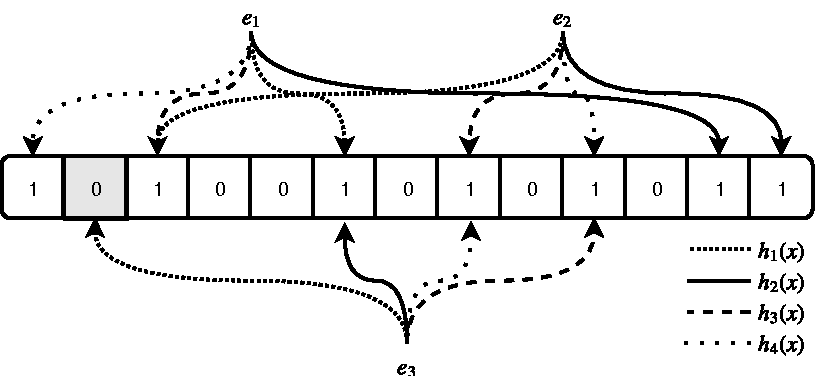
\includegraphics[width=1\textwidth]{./graph/bloom.pdf}
	\caption{Filtro Bloom}
	\label{fig:bloom}
	\medskip
	\small
	
	\parbox{13.1cm}{La imagen muestra un filtro de Bloom luego que los elementos $e_1$ y $e_2$ fueron insertados. El elemento $e_3$ no se encuentra en el conjunto dado que al menos uno de los bits a los que apuntan las funciones de hash es $0$. La pertenencia de un elemento $e'$ al conjunto puede ser reportada erróneamente si las $k$ funciones de hash $h_i(e')$ apuntan a bits con valor $1$.}
	
\end{figure}

La ventaja principal de los filtros de \textit{Bloom} es evidente cuando se la compara con otras estructuras de datos usadas para implementar \textit{sets} (listas, tablas de \textit{hash}, arboles binarios de búsqueda, etc). Estas requieren almacenar el elemento en sí, lo cual puede requerir una cantidad pequeña de bits si los elementos son números enteros, hasta un número arbitrario de bits en el caso que los elementos sean \textit{strings}. Sin embargo, estas estructuras probabilísticas no necesitan almacenar el elemento en sí, y tampoco introducen el \textit{overhead} generado por los punteros que utilizan las estructuras enlazadas como las listas.

La cantidad óptima de funciones de hash $k$ puede deducirse como sigue. Sea la probabilidad que uno de los bits del filtro de \textit{Bloom} sea 0:

\begin{equation}
	\mathcal{P} [h_i(x)=0 ] = (1- \frac{1}{m})^{kn} \approx e ^ {-\frac{kn}{m}} = p
\end{equation}

La probabilidad de tener un falso positivo está dada por:
\begin{equation}
	(1 - e ^ {-\frac{kn}{m}})^k = (1 - p)^k = \varepsilon
\end{equation}

El valor óptimo de $\hat{k}$ se obtiene al minimizar la ecuación anterior, de forma que $\hat{k} = \ln(2) \frac{m}{n}$. La probabilidad de falso positivo está dada por la fórmula\cite{Bloom:1970:STH:362686.362692}:
\begin{equation}
	\varepsilon = (0.5) ^ {\hat{k}} = (0.6185)^{\frac{m}{n}}
\end{equation}

Un filtro de \textit{Bloom} con un error de $1\%$ y un valor óptimo de $k$ requiere alrededor de $10$ bits por elemento, sin importar el tamaño del elemento. Para reducir el error a un $0.1\%$ se deben emplear alrededor de $15$ bits.

\

Esta estructura de datos, en su versión clásica, no resuelve el problema de los elementos frecuentes (para esto se utiliza una variante llamada \textit{filtros de conteo}). Sin embargo, resulta útil para ganar intuición: los algoritmos de \textit{sketches} son similares a los filtros de \textit{Bloom} en el uso de las funciones de hash para representar conjuntos de elementos. Utiliza estructuras auxiliares que permiten aproximar el número de elementos que fueron vistos en el \textit{stream} de datos.  

\subsubsection{CountMin Sketch}

Los \textit{sketches} son menos conocidos que los filtros \textit{Bloom} pero comparten ciertas similitudes. Son estructuras de datos que permiten sumarizar un \textit{stream} de datos y pueden utilizarse para resolver el problema de los elementos frecuentes. Esto puede ser llevado a cabo usando menos espacio del que se utilizaría almacenando un contador por elemento, pero permitiendo que los contadores tengan cierto error en algunas ocasiones. Si bien existen otras implementaciones cómo Count Sketch\cite{Charikar:2002:FFI:646255.684566} y AMS Sketch\cite{Alon:1996:SCA:237814.237823}, CountMin Sketch es una estructura de datos mas sencilla, fácil de construir, que asegura muy buenas garantías de precisión cuando se hacen consultas sobre los datos procesados.

Un CM Sketch es simplemente una matriz de contadores de $d$ filas y $w$ columnas, cuyo valor inicial es $0$. Además, se escogen aleatoriamente $d$ funciones de hash de una familia de funciones de hash independientes de a pares (ver Sección \ref{k_independent_hash_func}):
\begin{equation*}
	h_1 \dots h_d: \{1 \dots n\} \rightarrow \{1 \dots w\}
\end{equation*}

Una vez que $w$ y $d$ son definidos, el espacio alocado no varía: la estructura de datos es representada por $wd$ contadores y $d$ funciones de hash (que puede ser representado en $O(1)$ variables\cite{Motwani:1995:RA:211390}).


Sea $\mathbf{a}$ un vector de dimensión $n$ cuyo estado en el tiempo $t$ es $\mathbf{a}(t)=[a_1(t), a_2(t), \dots, a_n(t)]$. Inicialmente $\mathbf{a}$ es el vector $\mathbf{0}$, es decir $a_i(0)=0 \ \forall i$. Las actualizaciones a los elementos de $\mathbf{a}$ se representan mediante un \textit{stream} de tuplas. De forma general, la tupla $(i_t, c_t)$ representa el $t$-ésimo elemento procesado\footnote{Para conteo de elementos $c_t=1$.}:

\begin{gather*}
a_{i_t}(t)=a_{i_t}(t-1) + c_t\\
a_{i_{t'}}(t)=a_{i_{t'}}(t-1) \ \forall t' \neq t 
\end{gather*}

Por cada elemento del \textit{stream} se calculan las $d$ posiciones de los contadores mediante $(j, h_j(i_t))$ para $j \in \{0,1 \dots d-1 \}$ y se los actualiza con el valor de $c_t$:

\begin{figure}[htp]
	\centering
	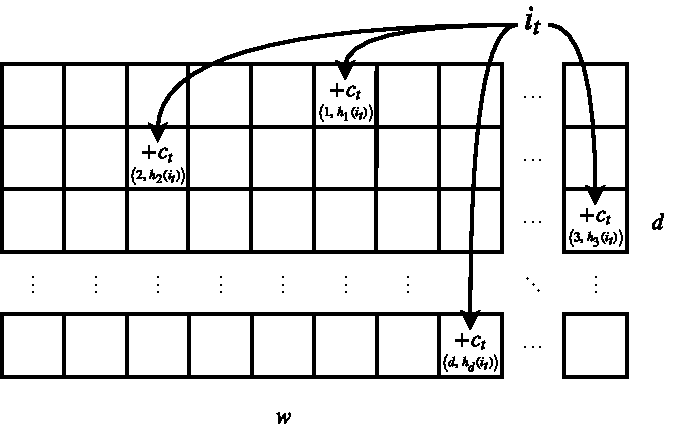
\includegraphics[width=1\textwidth]{./graph/cm_sketch.pdf}
	\caption{COUNTMIN Sketch}
	\label{fig:cm_sketch}
	\medskip
	\small
	
	\parbox{13.1cm}{La figura muestra el proceso de actualización de un sketch COUNTMIN. Se calcula la posición de los contadores para cada fila evaluando la función de hash correspondiente con el elemento $i_t$. Luego, los contadores de las posiciones $(j, h_j(i_t))$ se actualizan con el valor de $c_t$.}
	
\end{figure}

Formalmente, dado $(i_t, c_t)$, se realizan las siguientes modificaciones:
\begin{equation}
	\forall \ 0 \leq j < d: CM[j, h_j(i_t)] \leftarrow  CM[j, h_j(i_t)] + c_t
\end{equation}

Como computar cada función de hash es $O(1)$, el proceso completo de actualización es $O(d)$ (independiente de $w$). Por este motivo, esta estructura de datos es ideal para procesar datos que son generados a gran velocidad.

Los sketches pueden ser usados para estimar el valor de $a_i$ en cualquier instante de tiempo. El proceso de consulta es similar al de actualización: dado un $i_t$, podemos estimar el valor $a_i$ de la siguiente forma:

\begin{equation}
	\hat{a}_i = \min_{\{0,1  \dots d-1 \}}CM[j, h_j(i_t)]
\end{equation}

\paragraph{Teorema} Sea $w=\lceil e / \varepsilon \rceil$ y $d=\lceil \ln (1 / \delta) \rceil$, la estimación $\hat{a}_i$ tiene las siguientes garantías: $a_i \leq \hat{a}_i$ y, con probabilidad al menos $1-\delta$:
\begin{equation}
	\hat{a}_i = a_i + \varepsilon ||\mathbf{a}||_1
\end{equation}
El desarrollo y la demostración de este teorema puede encontrarse en \cite{Cormode:2005:IDS:1073713.1073718}. Es importante remarcar cómo se comporta la estimación de los contadores cuando variamos el tamaño de la matriz. A medida que agregamos filas, el valor de $\delta$ tiene que disminuir, por lo que la probabilidad que $\hat{a}_i$ este acotado como se muestra en el teorema aumenta. Además, cuando la cantidad de columnas $w$ aumenta, el valor de $\varepsilon$ tiene que disminuir, haciendo que la estimación $\hat{a}_i$ se aproxime cada vez más a el valor real.

\subsubsection{Extendiendo los sketches: LD-Sketch}
A lo largo de los años, la comunidad ha estudiado y publicado numerosas mejoras a estas estructuras de datos. En particular, los LD-Sketch \cite{Huang:2015:HLD:2839515.2839568} hacen uso de las técnicas de conteo tratadas en \ref{tecnicas_conteo} para aumentar los sketches, mejorando así la precisión de las estimaciones. Además, sus autores proponen una arquitecta distribuida, donde cada objeto puede ser almacenado y actualizado en un equipos diferentes, permitiendo procesar un conjunto de sketches en paralelo, brindando redundancia y la posibilidad de escalar el sistema para hacer frente a volúmenes masivos de datos.

La idea principal es hacer que cada celda del sketch utilice una técnica de conteo para mantener conjunto de potenciales elementos anómalos en una lista asociativa. La detección local\footnote{Únicamente se trabajará con detección local. La detección distribuida reduce la cantidad de falsos positivos combinando los resultados de varios sketches procesados en paralelo.} garantiza la ausencia de falsos negativos y permite identificar elementos anómalos (con algunos falsos positivos) en un único nodo de cómputo.

Para la técnica de conteo FREQUENT\ref{FREQUENT} el siguiente lema muestra la cota de error para el valor estimado\cite{Misra1982143}:

\paragraph{Lema 1} Sea un stream de datos $\{ t_i = (j, I_i)\}$ con $I_i=1$, $S(x)$ representa la cantidad de elementos $x$ que ocurrieron en una época y $U$ todos los elementos procesados en esa época. Si $j$ se mantiene en $A$, entonces $A[j] \leq S(x) \leq A[j] + \frac{U}{l}$. Si $x$ no se mantiene en $A$, su valor estimado es $0$ y $0 \leq S(x) \leq \frac{U}{l}$

Las técnicas basadas en conteo pueden identificar todos los \textit{heavy hitters} (sin incurrir en falsos negativos) que excedan el umbral $\phi = \frac{U}{l}$ comprobando si un elemento tiene un contador positivo en la lista asociativa.








\section{Detección de anomalías}
Cómo se mencionó anteriormente, existen muchos indicadores de escenarios que pueden tener impacto negativos en una infraestructura de red. Una práctica muy común en la etapa reconocimiento\footnote{El modelo de seguridad informática llamado \textit{cyber kill chain} describe las 7 etapas que todo atacante ejecuta para lograr su objetivo.\cite{hutchins2011intelligence}}, por donde comienzan todos los ataques, es el escaneo de puertos; uno o varios atacantes envían paquetes a un rango de puertos para determinar que servicios están activos, generando así grandes volúmenes de tráfico en la red. Otro escenario crítico es el de \textit{command and control (C2)} en donde el atacante tiene control de un conjunto de equipos ya infectados y utiliza sus recursos para atacar otro objetivo. Esto también genera tráfico anómalo y es un indicador crítico ante el cual se deben tomar medidas inmediatamente. Otro indicador son las fluctuaciones repentinas en los flujos de datos, que pueden indicar ataques de denegación de servicio (DoS).

La lista de ataques podría extenderse, pero de forma general pueden definirse dos tipos de comportamientos anómalos que son útiles para identificar amenazas. Para esto es necesario modelar el problema bajo el modelo de \textit{data streaming}.

\subsection{Modelado del problema}\label{modelado}

Consideremos los segmento TCP que atraviesa un punto de acceso; estos pueden ser representados como un \textit{stream} de eventos, donde cada elemento es una tupla $(x, v_x)$. El elemento $x$ pertenece a un dominio $T=\{0,1,2, \dots, n-1\}$ con $|T|=n$, y $v_x$ es un valor asociado a $x$. Para el caso de detección de eventos en tráfico de red, cada \textit{key} $x$ identifica un segmento TCP y está formado por la 5-tupla IP de origen, IP de destino, puerto de origen, puerto de destino y protocolo. El valor $v_x=1$ representa cantidad de paquetes identificados por $x$. Dado un \textit{stream} de eventos o \textit{keys}, definimos \textbf{\textit{heavy hitters}} como aquellos elementos que aparece más frecuentemente en el \textit{stream} de eventos. Los \textbf{\textit{heavy changers}} son aquellos elementos que presentan inconsistencias significativas entre el comportamiento observado y el comportamiento normal del flujo de datos (el cual se basa en lo ocurrido en el pasado) en un período de tiempo acotado\cite{Tong:2016:HTS:2927964.2927977}. 
En un algoritmo de detección de \textbf{\textit{heavy keys}}\footnote{Este término suele utilizase para referirse a ambos tipos de anomalías} típicamente se realizan dos procedimientos: en el primero, llamado de actualización, el valor de cada elemento es procesado y se almacenan los resultados en una estructura de datos; en el segundo, de detección, se examina la estructura de datos en cada época y se determinan los \textit{heavy keys}.

Para detectar \textit{heavy keys} se realizan estimaciones de frecuencias en ventanas de tiempo o épocas. En cada época, sea $S(x)$ la suma de los valores $v_x$ del elemento $x$. Sea $D(x)$ la diferencia (en valor absoluto) de $S(x)$ en la época actual y la anterior. Además, sea $U=\sum_{x \in T} S(x)$ la suma total de todos los elementos $x$ en una época. El problema de detectar \textit{heavy keys} consiste en encontrar aquellos elementos cuya suma o diferencias excedan, en valor absoluto, al parámetro $\phi$ en una época. Formalmente, definimos cómo \textit{heavy hitters} a aquellos elementos $x$ con $S(x) \geq \phi_1$, y \textit{heavy changers} a los elementos $x$ con $D(x) \geq \phi_2$. En adelante, referiremos indistintamente a los parámetros $\phi_1$ y $\phi_2$ como $\phi$, teniendo en cuenta que pueden ser diferentes.

\

Podemos encontrar los \textit{heavy hitters} resolviendo el problema de los elementos frecuentes. Los \textit{heavy changers} pueden ser identificados realizando estimaciones de frecuencia de los diferentes elementos para ventanas de tiempo adyacentes. Dada la naturaleza del problema es necesario implementar soluciones eficientes en el costo de cómputo como en costo de memoria.


\newpage
\section{Apéndices}

\paragraph{Funciones de hash k-independientes}\label{k_independent_hash_func}
El objetivo de las funciones de hash es asociar elementos de un gran conjunto a otro más pequeño. En las estructuras de datos probabilísticas, usualmente es deseable que los códigos de hash se comporten de manera aleatoria, pues si se usan funciones de hash determinísticas un adversario podría escoger un conjunto de datos con las mismas pre-imágenes. Ademas, es posible que la elección de una función de hash determinística sea una mala elección para un conjunto de entrada dado (muchas colisiones): escoger aleatoriamente funciones de hash de una familia de funciones evita este problema dado que si bien puede escogerse una función con esta característica, lo más probable es que solo sea un caso asilado.
Existe una familia de funciones que asegura baja probabilidad de colisiones para un conjunto dado de elementos y comportamiento uniforme en la distribución de las pre-imágenes de los elementos\cite{WEGMAN1981265}.

La familia de funciones $\mathcal{H} = \{h: U \rightarrow \{0, 1, \dots, m-1\} \}$ es \textit{k-independiente} si para $k$ elementos diferentes $(x_1, x_2, \dots, x_k)$ y $k$ códigos de hash (no necesariamente diferentes) $(y_1, y_2, \dots, y_k) \in \{0, 1, \dots, m-1 \}$ tenemos que:

\begin{equation}
\mathcal{P}[h(x_1) = y_1 \hat{\ } \ h(x_2) = y_2 \ \dots \  h(x_k) = y_k] = \frac{1}{m^k}
\end{equation}

La ecuación anterior puede interpretarse de dos maneras:
\begin{itemize}
	\item Para un elemento dado $x \in U$, $h(x)$ se distribuye de forma uniforme en $\{0, 1, \dots, m-1 \}$ siempre que $h$ se elija aleatoriamente de $H$.
	\item Para un conjunto dado de elementos $(x_1, x_2, \dots, x_k) \in U$, si $h$ se elije aleatoriamente de $H$, entonces $h(x_1), h(x_2), \dots, h(x_k)$ son variables aleatorias independientes.
\end{itemize}


\newpage
\nocite{*}
\printbibliography
\end{document}

